%%%%%%%%%%%%%%%%%%%%%%%%%%%%%%%%%%%%%%%%%
% Friggeri Resume/CV
% XeLaTeX Template
% Version 1.0 (5/5/13)
%
% This template has been downloaded from:
% http://www.LaTeXTemplates.com
%
% Original author:
% Adrien Friggeri (adrien@friggeri.net)
% https://github.com/afriggeri/CV
%
% License:
% CC BY-NC-SA 3.0 (http://creativecommons.org/licenses/by-nc-sa/3.0/)
%
% Important notes:
% This template needs to be compiled with XeLaTeX and the bibliography, if used,
% needs to be compiled with biber rather than bibtex.
%
%%%%%%%%%%%%%%%%%%%%%%%%%%%%%%%%%%%%%%%%%

\documentclass[print]{friggeri-cv} % Add 'print' as an option into the square bracket to remove colors from this template for printing
\usepackage{fontspec}
\usepackage{fontawesome}

\begin{document}

\header{James}{McCormac}{Curriculum Vitae} % Your name and current job title/field

%----------------------------------------------------------------------------------------
%	SIDEBAR SECTION
%----------------------------------------------------------------------------------------

\begin{aside} % In the aside, each new line forces a line break
\vspace{0.35cm}~
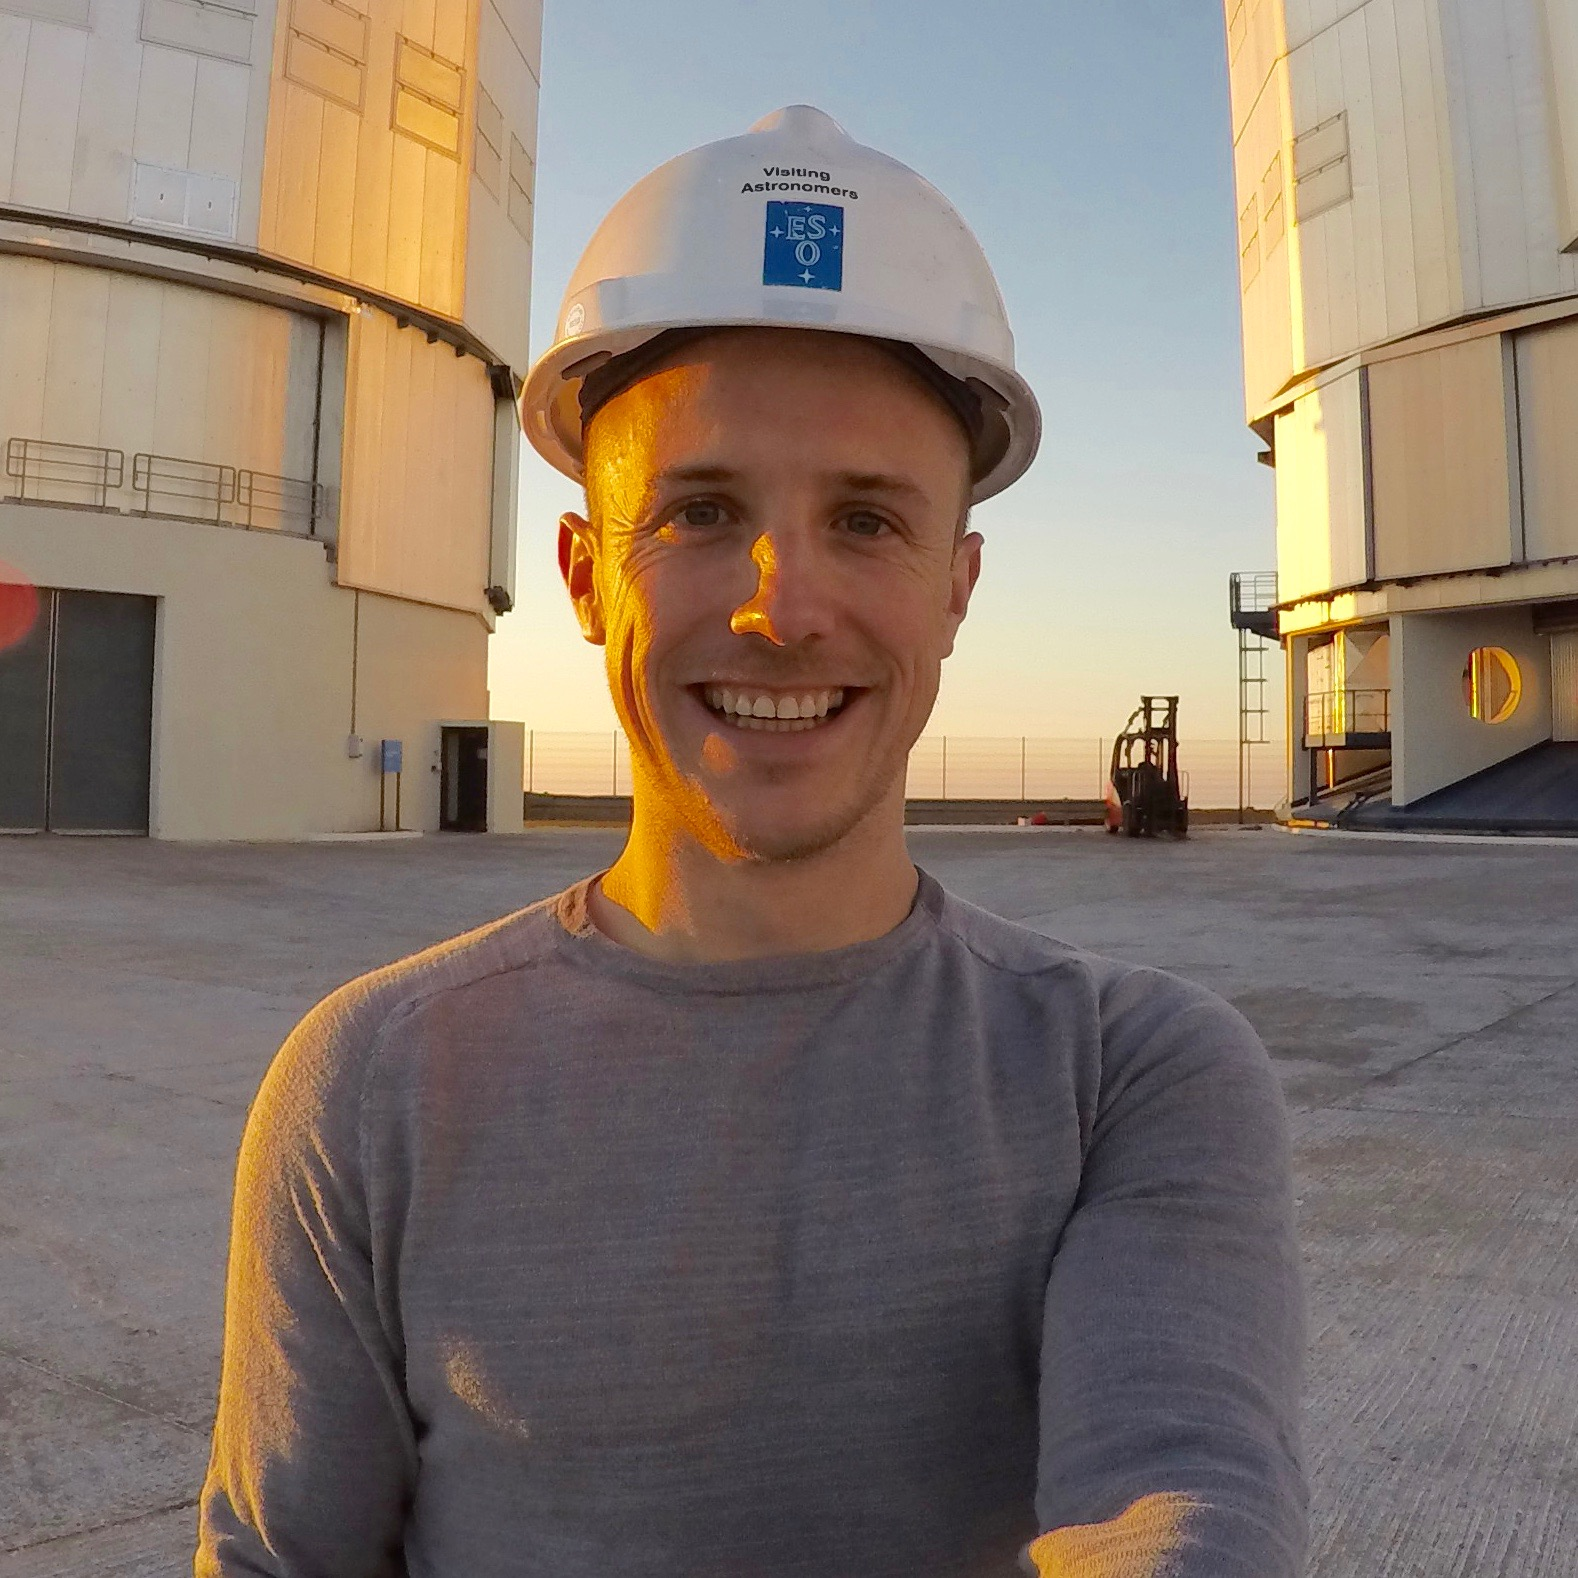
\includegraphics[width=4.0cm]{CV_Photo.jpg}
~
\section{Contact}
Department of Physics
University of Warwick
Gibbet Hill Road
Coventry
CV4 7AL
UK
~
{\bf mobile:} 
+44 77139 46903
{\bf work:} 
+44 24765 74211
{\bf email:}
{\small j.j.mccormac@warwick.ac.uk}
~
\section{Links}
{\small \faLinkedin~jmcc001}
{\small \faSkype~jmccormac01}
{\small \faGithub~jmccormac01}
{\small \faGlobe~jamesjmccormac.com}
~
\section{Languages}
English (Native)
Spanish (Fluent)
\section{Programming}
Python, C/C++
HTML, Javascript, 
PHP, CSS, MySQL,  
JQuery, AngularJS,
Flask, Git
\section{Computing}
Linux, Mac, Windows
IRAF, PyRAF, LaTex,
Microsoft Office
\end{aside}

%----------------------------------------------------------------------------------------
%	EDUCATION SECTION
%----------------------------------------------------------------------------------------

\section{Education}

\begin{entrylist}
%------------------------------------------------
\entry
{2008--2012}
{Doctor {\normalfont of Philosophy}}
{Queen's University Belfast, BT7 1NN, U.K.}
{\emph{The Next Generation of Transiting Exoplanet Surveys} \\ In my thesis I describe the design, construction, commissioning and testing of a prototype telescope for the Next Generation Transit Survey (NGTS), that I carried out between 2008 and 2010. I also describe the new, remotely operated 0.4m NITES telescope which I installed and commissioned on La Palma. I present the results from a 60 night survey for transiting exoplanets in the globular cluster M71 using NITES. Finally, I present a new science-frame autoguiding algorithm with sub-pixel precision, capable of autoguiding on defocused stars, DONUTS. I highlight the off and on-sky tests of DONUTS and explain why such an algorithm is essential for high-precision ground-based photometry.}
%------------------------------------------------
\entry
{2004--2008}
{MSci {\normalfont in Physics with Astrophysics}}
{Queen's University Belfast, BT7 1NN, U.K.}
{I obtained a first class honours degree in my 4 year Masters course at Queen's University. I was awarded the Raymond Greer prize for best overall MSci in 2008.}
\end{entrylist}

%----------------------------------------------------------------------------------------
%	WORK EXPERIENCE SECTION
%----------------------------------------------------------------------------------------

\section{Experience}

\begin{entrylist}
%------------------------------------------------
\entry
{2014--2018}
{University of Warwick}
{Gibbet Hill Road, Coventry, CV4 7AL}
{\emph{Postdoctoral Research Fellow: NGTS project}\\
My current 4-year postdoc is primarily based on the installation, commissioning and operation of the full NGTS facility at ESO Paranal, Chile. NGTS consists of 12 robotic 20cm red-optimised telescopes and aims to discover Neptune and super-Earth sized exoplanets. NGTS achieved first light with the first telescope in Jan 2015 and the facility reached full capacity (12 telescopes) in Feb 2016. We are currently confirming our first round of planet candidates with radial velocities from the CORALIE and HARPS spectrographs. I have written software and webpages used in the operation of the facility. I am also responsible for the semi-robotic 0.4m NITES telescope on La Palma, which I installed and commissioned during the final year of my Ph.D. NITES is typically used in exoplanet follow-up from the SuperWASP survey, of which I am also a member. I demonstrate in 1st year Python labs and in 2014 and 2015 I co-supervised 2 groups of final year masters students, both with projects based on NITES observations. In 2015 I began leading a scientific project to discover and characterise very large planets and brown dwarfs from the SuperWASP survey. Finally, I am also involved with the University of Warwick 1m telescope project and the new Gravitational wave Optical Transient Observatory (GOTO) project. } 
%------------------------------------------------
\entry
{2012--2014}
{Isaac Newton Group of Telescopes}
{Santa Cruz de La Palma, Canary Islands, Spain}
{\emph{Telescope Operator \& Support Astronomer}\\
My duties as a telescope operator involved providing expert support to visiting observers and minimising telescope downtime. As a support astronomer I was responsible for instrument setup, introducing visiting observers to the instruments and enabling them to complete their observations efficiently. I provided support for the ACAM, ISIS and LIRIS instruments on the WHT as well as supporting visiting instruments. I wrote numerous observing scripts in Python that increased efficiency at the observatory and are currently in use today. I also supervised a summer project student in 2013.
} 
\end{entrylist}
\begin{entrylist}
%------------------------------------------------
\entry
{2009--2010}
{Isaac Newton Group of Telescopes}
{Santa Cruz de La Palma, Canary Islands, Spain}
{\emph{Student Support Astronomer} \\
For almost 1.5 years during my Ph.D I worked as a student support astronomer at the 2.5m Isaac Newton Telescope on La Palma. I was responsible for setting up the WFC and IDS instruments (imaging and spectroscopy) and introducing visiting observers to the telescope and instruments subsequently enabling them to complete their observations efficiently.}
%------------------------------------------------
\end{entrylist}

%----------------------------------------------------------------------------------------
%	AWARDS SECTION
%----------------------------------------------------------------------------------------

\section{Awards}

\begin{entrylist}
%------------------------------------------------
\entry
{2013 \& 2014}
{Exceptional Performance Award}
{Isaac Newton Group of Telescopes}
{Award for exceptional performance in my previous position at the ING.}
\entry
{2008}
{Raymond Greer Award}
{Queen's University Belfast}
{Awarded each year for the best overall Physics MSci.}
\entry
{2008}
{Certificate of Entrepreneurial Studies}
{Queen's University Belfast}
{Awarded to the winners of an Entrepreneurial Studies competition.}

%------------------------------------------------
\end{entrylist}

%----------------------------------------------------------------------------------------
%	PUBLICATIONS SECTION
%----------------------------------------------------------------------------------------

\section{Publications}
\begin{entrylist}
\entry
{\small 2017}
{\small The Next Generation Transit Survey - Prototyping Phase}
{}
{\small McCormac, J., et al. 2017, PASP, 129, 972}
%------------------------------------------------
\entry
{\small 2016}
{\normalfont \small Rayleigh scattering in the transmission spectrum of HAT-P-18b}
{}
{\small Kirk, J., et al. 2016, ArXiv, 1611.06916}
%------------------------------------------------
\entry
{\small 2016}
{\normalfont \small WASP-92b, WASP-93b and WASP-118b: three new transiting close-in giant planets}
{}
{\small Hay, K.~L., et al. 2016,  MNRAS, 463, 3276}
%------------------------------------------------
\entry
{\small 2016}
{\normalfont \small The Astropy Problem}
{}
{\small Muna, D., et al. 2016, ArXiv, 1610.03159}
%------------------------------------------------
\entry
{\small 2016}
{\normalfont \small K2-30 b and K2-34 b: Two inflated hot Jupiters around solar-type stars}
{}
{\small Lillo-Box, J., et al. 2016, A\&A, 594, A50}
%------------------------------------------------
\entry
{\small 2016}
{\normalfont \small WASP-113b and WASP-114b, two inflated hot Jupiters with contrasting densities}
{}
{\small Barros, S.~C.~C., et al. 2016, A\&A, 593, A113}
%------------------------------------------------
\entry
{\small 2016}
{\normalfont \small The Next Generation Transit Survey Becomes Operational at Paranal}
{}
{\small West, R.~G., et al. ESO Messenger, 16, 10}
%------------------------------------------------
\entry
{\small 2016}
{\normalfont \small Supernova 2014J at M82 - II. Direct analysis of a middle-class Type Ia supernova}
{}
{\small Vallely, P., et al. 2016, MNRAS, 460, 1614}
%------------------------------------------------
\entry
{\small 2016}
{\normalfont \small WASP-86b and WASP-102b: super-dense versus bloated planets}
{}
{\small Faedi, F., et al. 2016, ArXiv, 1608.04225}
%------------------------------------------------
\entry
{\small 2016}
{\normalfont \small From Dense Hot Jupiter to Low Density Neptune: The Discovery of WASP-127b, WASP-136b and WASP-138b}
{}
{\small Lam, K.~W.~F., et al. 2016, ArXiv, 1607.07859}
%------------------------------------------------
\entry
{\small 2016}
{\normalfont \small K2-29 b/WASP-152 b: An Aligned and Inflated Hot Jupiter in a Young Visual Binary}
{}
{\small Santerne, A., et al. 2016,  ApJ, 824, 55}
%------------------------------------------------
\entry
{\small 2016}
{\normalfont \small EPIC212521166 b: a Neptune-mass planet with Earth-like density}
{}
{\small Osborn, H.~P., et al. 2016, ArXiv, 1605.04291}
%------------------------------------------------
\entry
{\small 2016}
{\normalfont \small K2 Variable Catalogue II: Machine Learning Classification of Variable Stars and Eclipsing Binaries in K2 Fields 0-4}
{}
{\small Armstrong, D.~J., et al. 2016, MNRAS, 456, 2260}
%------------------------------------------------
\entry
{\small 2016}
{\normalfont \small SN 2014J at M82: I. A middle-class type Ia supernova by all spectroscopic metrics}
{}
{\small Galbany, L., et al. 2016, MNRAS, 457, 525}
%------------------------------------------------
\end{entrylist}
\begin{entrylist}
\entry
{\small 2016}
{\normalfont \small Single Transit Candidates from K2: Detection and Period Estimation}
{}
{\small Osborn, H.~P., et al. 2016, MNRAS, 457, 2273}
%------------------------------------------------
\entry
{\small 2016}
{\normalfont \small WASP-135b: a highly irradiated, inflated hot Jupiter orbiting a G5V star}
{}
{\small Spake, J., et al. 2016, PASP, 128, 2}
%------------------------------------------------
\entry
{\small 2015}
{\normalfont \small Photodynamical mass determination of the multiplanetary system K2-19}
{}
{\small Barros, S.~C.~C., et al. 2015, MNRAS, 454, 4267}
%------------------------------------------------
\entry
{\small 2015}
{\normalfont \small Characterization of the K2-19 Multiple-transiting Planetary System via High-dispersion Spectroscopy, AO Imaging, and Transit Timing Variations}
{}
{\small Narita, N., et al. 2015, ApJ, 815, 47}
%------------------------------------------------
\entry
{\small 2015}
{\normalfont \small One of the closest exoplanet pairs to the 3:2 mean motion resonance: K2-19b and c}
{}
{\small Armstrong, D.~J., et al. 2015, A\&A, 582, A33}
%------------------------------------------------
\entry
{\small 2015}
{\normalfont \small K2 Variable Catalogue: Variable stars and eclipsing binaries in K2 campaigns 1 and 0}
{}
{\small Armstrong, D.~J., et al. 2015, A\&A, 579, A19}
%------------------------------------------------
\entry
{\small 2015}
{\normalfont \small Subaru and Swift observations of V652 Herculis: resolving the photospheric pulsation}
{}
{\small Jeffery, C.~S. et al. 2015, MNRAS, 447, 2836}
%------------------------------------------------
\entry
{\small 2014}
{\small The Next Generation Transit Survey Prototyping Phase}
{}
{\small McCormac, J, et al. 2014, RevMex Conference Series, 45, 98}
%------------------------------------------------
\entry
{\small 2014}
{\normalfont \small The EBLM project. II. A very hot, low-mass M dwarf in an eccentric and long-period, eclipsing binary system from the SuperWASP Survey}
{}
{\small G{\'o}mez Maqueo Chew, Y., et al. 2014, A\&A, 572, A50}
%------------------------------------------------
\entry
{\small 2014}
{\small A Search for Photometric Variability towards M71 with the Near-Infrared Transiting ExoplanetS Telescope}
{}
{\small McCormac, J., et al. 2014, MNRAS, 438, 3383}
%------------------------------------------------
\entry
{\small 2014}
{\normalfont \small A Window on Exoplanet Dynamical Histories: Rossiter-McLaughlin Observations of WASP-13b and WASP-32b}
{}
{\small Brothwell, R. D., et al. 2014, ArXiv 1403.4095}
%------------------------------------------------
\entry
{\small 2014}
{\normalfont \small Next Generation Transit Survey}
{}
{\small Wheatley, P.~J., et al. 2014, Exploring the Formation and Evolution of Planetary Systems, Proceedings of the International Astronomical Union, 299, 311}
%------------------------------------------------
\entry
{\small 2013}
{\normalfont \small Discovery of WASP-65b and WASP-75b: Two hot Jupiters without highly inflated radii}
{}
{\small G{\'o}mez Maqueo Chew, Y., et al. 2013, A\&A, 559, A36}
%------------------------------------------------
\entry
{\small 2013}
{\normalfont \small Discovery of Five Probable Novae in M81}
{}
{\small Hornoch, K., et al. 2013, The Astronomer's Telegram, 5489, 1}
%------------------------------------------------
\entry
{\small 2013}
{\normalfont \small Discovery of Two Apparent Novae in M81}
{}
{\small Hornoch, K., McCormac, J., Vaduvescu, O., 2013, The Astronomer's Telegram, 5109, 1}
%------------------------------------------------
\entry
{\small 2013}
{\small DONUTS: A Science Frame Autoguiding Algorithm with Sub-Pixel Precision, Capable of Guiding on Defocused Stars}
{}
{\small McCormac, J., et al. 2013, PASP, 125, 548}
%------------------------------------------------
\entry
{\small 2013}
{\normalfont \small The Next Generation Transit Survey (NGTS)}
{}
{\small Wheatley, P.~J., et al. 2013, European Physical Journal Web of Conferences, 47, 13002}
%------------------------------------------------
\entry
{\small 2013}
{\normalfont \small WASP-54b, WASP-56b, and WASP-57b: Three new sub-Jupiter mass planets from SuperWASP}
{}
{\small Faedi, F., et al. 2013, A\&A, 551, A73}
%------------------------------------------------
\entry
{\small 2013}
{\normalfont \small WASP-52b, WASP-58b, WASP-59b, and WASP-60b: Four new transiting close-in giant planets}
{}
{\small H{\'e}brard, G., et al. 2013, A\&A, 549, A134}
%------------------------------------------------
\entry
{\small 2012}
{\normalfont \small A hot Uranus transiting the nearby M dwarf GJ 3470. Detected with HARPS velocimetry. Captured in transit with TRAPPIST photometry}
{}
{\small Bonfils, X., et al. 2012, A\&A, 546, A27}
%------------------------------------------------
\entry
{\small 2012}
{\normalfont \small NGTS: a robotic transit survey to detect Neptune and super-Earth mass planets}
{}
{\small Chazelas, B., et al. 2012, SPIE Conference Series, 8444}
%------------------------------------------------
\entry
{\small 2012}
{\normalfont \small A transiting companion to the eclipsing binary KIC002856960}
{}
{\small Armstrong, D., et al. 2012, A\&A, 545, L4}
%------------------------------------------------
\end{entrylist}
\begin{entrylist}
\entry
{\small 2011}
{\normalfont \small WASP-35b, WASP-48b, and HAT-P-30b/WASP-51b: Two New Planets and an Independent Discovery of a HAT Planet}
{}
{\small Enoch, B., et al. 2011, AJ, 142, 86}
%------------------------------------------------
\entry
{\small 2011}
{\normalfont \small WASP-40b: Independent Discovery of the 0.6 M Transiting Exoplanet HAT-P-27b}
{}
{\small Anderson, D.~R., et al. 2011, PASP, 123, 555}
%------------------------------------------------
\entry
{\small 2011}
{\normalfont \small Independent Discovery of the Transiting Exoplanet HAT-P-14b}
{}
{\small Simpson, E.~K., et al. 2011, AJ, 141, 161}
%------------------------------------------------
\entry
{\small 2011}
{\normalfont \small WASP-37b: A 1.8 M$_{J}$ Exoplanet Transiting a Metal-poor Star}
{}
{\small Simpson, E.~K., et al. 2011, AJ, 141, 8}
%------------------------------------------------
\entry
{\small 2011}
{\normalfont \small WASP-38b: a transiting exoplanet in an eccentric, 6.87d period orbit}
{}
{\small Barros, S.~C.~C., et al. 2011, A\&A, 525, A54}
%------------------------------------------------
\end{entrylist}

%----------------------------------------------------------------------------------------
%	PUBLICATIONS SECTION
%----------------------------------------------------------------------------------------

\section{Journal Referee}
\begin{entrylist}
\entry
{\small 2015}
{\small Monthly Notices of the Royal Astronomical Society}
{}
{\small Technical publication on a new scientific instrument}

%------------------------------------------------
\end{entrylist}

%----------------------------------------------------------------------------------------
%	CONFERENCES SKILLS SECTION
%----------------------------------------------------------------------------------------

\section{Conferences}

\begin{entrylist}
%------------------------------------------------
\entry
{\small 2016}
{\small Oral Presentation}
{\small European Southern Observatory, Paranal, Chile}
{\small Presented an NGTS project overview to ESO staff at Paranal.}
%------------------------------------------------
\entry
{\small 2016}
{\small Oral Presentation}
{\small National Astronomy Meeting, Nottingham, UK}
{\small Presented the current status of the NGTS project and our first planet candidates to the professional community.}
%------------------------------------------------
\entry
{\small 2016}
{\small Poster}
{\small UK Exoplanet Meeting, Exeter, UK}
{\small Presented the current status of the NGTS project.}
%------------------------------------------------
\entry
{\small 2015}
{\small Oral Presentation}
{\small European Week of Astronomy and Space Science (EWASS), Tenerife}
{\small Presented a technical overview of the NGTS facility.}
%------------------------------------------------
\entry
{\small 2015}
{\small Poster}
{\small UK Exoplanet Meeting, Warwick, UK}
{\small Presented an NGTS project overview poster.}
%------------------------------------------------
\entry
{\small 2013}
{\small Oral Presentation}
{\small Third Workshop on Robotic Autonomous Observatories, Malaga}
{\small Presented the results from the NGTS prototyping phase to the amateur and professional community.}
%------------------------------------------------
\entry
{\small 2013}
{\small Oral Presentation}
{\small Isaac Newton Group of Telescopes, La Palma}
{\small Presented the research I conducted during my Ph.D to the staff at the ING, Nordic Optical and Mercator telescopes.}
%------------------------------------------------
\entry
{\small 2010}
{\small Attended}
{\small Royal Astronomical Society, London}
{\small Science with the William Herschel Telescope 2010-2020 workshop.}
%------------------------------------------------
\entry
{\small 2008}
{\small Attended}
{\small Royal Observatory, Edinburgh}
{\small ROE Workshop 2008: Habitability in Our Galaxy}
%------------------------------------------------
\end{entrylist}

%----------------------------------------------------------------------------------------
%	INTERESTS SECTION
%----------------------------------------------------------------------------------------
\section{Interests}

{\small \textbf{Professional:} Observational astronomy, extrasolar planets, photometry, image processing, data analysis, telescope construction and maintenance, computer programming, scripting, back/front end web development, scientific writing and public outreach. I am an advocate of open source programming and have made minor contributions to several open source projects (Astropy/CCDPROC, fswebcam and CERES), activity of which can be seen on Github. I have submitted my open source autoguiding and image alignment package DONUTS to Astropy as an affiliated package.}\\
{\small \textbf{Personal:} Trail running and photography.}

%----------------------------------------------------------------------------------------
%	REFERENCES SECTION
%----------------------------------------------------------------------------------------

\section{References}
{\small  Available on request}

\end{document}
